\section{Memory Organization}
\label{sec:memory_organization}
\subsection{Data Memory}
\label{ssec:data_memory}

\subsubsection{Memory interface}
\label{sssec:memory_interface}
\begin{itemize}
   \item Read/write cycles take only one clock period.
   \item Memory is organized in big-endian format.
   \item No long-data transfer (64 bits) is supported.
   \item Only aligned data is supported:
   \begin{itemize}
      \item A byte data can be located in any address.
      See figure \ref{fig:byte_alignment}.
      \item A half data can only be located in even addresses.
      See figure \ref{fig:half_alignment}.
      \item A word data can only be located in addresses multiple of 4.
      See figure \ref{fig:word_alignment}.
   \end{itemize}
   Read table \ref{tbl:dm_alignemnt}
\end{itemize}

\begin{table}
\begin{center}
\begin{tabu} to \textwidth {|X[c]|X[c]|X[2,c]|}
\hline
\textbf{Data type} & \textbf{Size} & \textbf{Address aligment condition} \\
\hline
\hline
Byte &  8 bits & xx...xxxx \\
\hline
Half & 16 bits & xx...xxx0 \\
\hline
Word & 32 bits & xx...xx00 \\
\hline
\end{tabu}

\caption{Data Memory Address Alignment Condition.}
\label{tbl:dm_alignemnt}
\end{center}
\end{table}

\begin{figure}
\begin{center}
\begin{bytefield}[bitwidth=0.9em]{40}
   \bitbox[]{8}{} & \bitbox[]{8}{+0} & \bitbox[]{8}{+1} & \bitbox[]{8}{+2} & \bitbox[]{8}{+3}\\
   \bitbox[]{8}{}
      & \bitbox[]{1}{\texttt{7}} & \bitbox[]{1}{\texttt{}} & \bitbox[]{1}{\texttt{}} & \bitbox[]{1}{\texttt{}}
      & \bitbox[]{1}{\texttt{}}  & \bitbox[]{1}{\texttt{}} & \bitbox[]{1}{\texttt{}} & \bitbox[]{1}{\texttt{0}}
      & \bitbox[]{1}{\texttt{7}} & \bitbox[]{1}{\texttt{}} & \bitbox[]{1}{\texttt{}} & \bitbox[]{1}{\texttt{}}
      & \bitbox[]{1}{\texttt{}}  & \bitbox[]{1}{\texttt{}} & \bitbox[]{1}{\texttt{}} & \bitbox[]{1}{\texttt{0}}
      & \bitbox[]{1}{\texttt{7}} & \bitbox[]{1}{\texttt{}} & \bitbox[]{1}{\texttt{}} & \bitbox[]{1}{\texttt{}}
      & \bitbox[]{1}{\texttt{}}  & \bitbox[]{1}{\texttt{}} & \bitbox[]{1}{\texttt{}} & \bitbox[]{1}{\texttt{0}}
      & \bitbox[]{1}{\texttt{7}} & \bitbox[]{1}{\texttt{}} & \bitbox[]{1}{\texttt{}} & \bitbox[]{1}{\texttt{}}
      & \bitbox[]{1}{\texttt{}}  & \bitbox[]{1}{\texttt{}} & \bitbox[]{1}{\texttt{}} & \bitbox[]{1}{\texttt{0}} \\
   \bitbox[]{8}{\texttt{0x00000000}} & \bitbox{8}{Byte} & \bitbox{8}{Byte} & \bitbox{8}{Byte} & \bitbox{8}{Byte}\\
   \bitbox[]{8}{\texttt{0x00000004}} & \bitbox{8}{Byte} & \bitbox{8}{Byte} & \bitbox{8}{Byte} & \bitbox{8}{Byte}\\
   \bitbox[]{8}{\texttt{0x00000008}} & \bitbox{8}{Byte} & \bitbox{8}{Byte} & \bitbox{8}{Byte} & \bitbox{8}{Byte}\\
   \bitbox[]{8}{\texttt{0x0000000C}} & \bitbox{8}{Byte} & \bitbox{8}{Byte} & \bitbox{8}{Byte} & \bitbox{8}{Byte}\\
   \bitbox[]{8}{}                    & \bitbox[lrt]{32}{} \\
   \bitbox[]{8}{}                    & \bitbox[lr]{32}{$\vdots$} \\
   \bitbox[]{8}{}                    & \bitbox[lrb]{32}{} \\
   \bitbox[]{8}{\texttt{0xFFFFFFFF}} & \bitbox{8}{Byte} & \bitbox{8}{Byte} & \bitbox{8}{Byte} & \bitbox{8}{Byte}\\
\end{bytefield}
\end{center}
\caption{Byte data type aligment.}
\label{fig:byte_alignment}
\end{figure}

\begin{figure}
\begin{center}
\begin{bytefield}[bitwidth=0.9em]{40}
   \bitbox[]{8}{} & \bitbox[]{8}{+0} & \bitbox[]{8}{+1} & \bitbox[]{8}{+2} & \bitbox[]{8}{+3}\\
   \bitbox[]{8}{}
      & \bitbox[]{1}{\texttt{7}} & \bitbox[]{1}{\texttt{}} & \bitbox[]{1}{\texttt{}} & \bitbox[]{1}{\texttt{}}
      & \bitbox[]{1}{\texttt{}}  & \bitbox[]{1}{\texttt{}} & \bitbox[]{1}{\texttt{}} & \bitbox[]{1}{\texttt{0}}
      & \bitbox[]{1}{\texttt{7}} & \bitbox[]{1}{\texttt{}} & \bitbox[]{1}{\texttt{}} & \bitbox[]{1}{\texttt{}}
      & \bitbox[]{1}{\texttt{}}  & \bitbox[]{1}{\texttt{}} & \bitbox[]{1}{\texttt{}} & \bitbox[]{1}{\texttt{0}}
      & \bitbox[]{1}{\texttt{7}} & \bitbox[]{1}{\texttt{}} & \bitbox[]{1}{\texttt{}} & \bitbox[]{1}{\texttt{}}
      & \bitbox[]{1}{\texttt{}}  & \bitbox[]{1}{\texttt{}} & \bitbox[]{1}{\texttt{}} & \bitbox[]{1}{\texttt{0}}
      & \bitbox[]{1}{\texttt{7}} & \bitbox[]{1}{\texttt{}} & \bitbox[]{1}{\texttt{}} & \bitbox[]{1}{\texttt{}}
      & \bitbox[]{1}{\texttt{}}  & \bitbox[]{1}{\texttt{}} & \bitbox[]{1}{\texttt{}} & \bitbox[]{1}{\texttt{0}} \\
   \bitbox[]{8}{\texttt{0x00000000}} & \bitbox[ltb]{8}{Byte 1} & \bitbox[rtb]{8}{Byte 0} & \bitbox[ltb]{8}{Byte 1} & \bitbox[rtb]{8}{Byte 0}\\
   \bitbox[]{8}{\texttt{0x00000004}} & \bitbox[ltb]{8}{Byte 1} & \bitbox[rtb]{8}{Byte 0} & \bitbox[ltb]{8}{Byte 1} & \bitbox[rtb]{8}{Byte 0}\\
   \bitbox[]{8}{\texttt{0x00000008}} & \bitbox[ltb]{8}{Byte 1} & \bitbox[rtb]{8}{Byte 0} & \bitbox[ltb]{8}{Byte 1} & \bitbox[rtb]{8}{Byte 0}\\
   \bitbox[]{8}{\texttt{0x0000000C}} & \bitbox[ltb]{8}{Byte 1} & \bitbox[rtb]{8}{Byte 0} & \bitbox[ltb]{8}{Byte 1} & \bitbox[rtb]{8}{Byte 0}\\
   \bitbox[]{8}{}                    & \bitbox[lrt]{32}{} \\
   \bitbox[]{8}{}                    & \bitbox[lr]{32}{$\vdots$} \\
   \bitbox[]{8}{}                    & \bitbox[lrb]{32}{} \\
   \bitbox[]{8}{\texttt{0xFFFFFFFF}} & \bitbox[ltb]{8}{Byte 1} & \bitbox[rtb]{8}{Byte 0} & \bitbox[ltb]{8}{Byte 1} & \bitbox[rtb]{8}{Byte 0}\\
\end{bytefield}
\end{center}
\caption{Half data type aligment.}
\label{fig:half_alignment}
\end{figure}

\begin{figure}
\begin{center}
\begin{bytefield}[bitwidth=0.9em]{40}
   \bitbox[]{8}{} & \bitbox[]{8}{+0} & \bitbox[]{8}{+1} & \bitbox[]{8}{+2} & \bitbox[]{8}{+3}\\
   \bitbox[]{8}{}
      & \bitbox[]{1}{\texttt{7}} & \bitbox[]{1}{\texttt{}} & \bitbox[]{1}{\texttt{}} & \bitbox[]{1}{\texttt{}}
      & \bitbox[]{1}{\texttt{}}  & \bitbox[]{1}{\texttt{}} & \bitbox[]{1}{\texttt{}} & \bitbox[]{1}{\texttt{0}}
      & \bitbox[]{1}{\texttt{7}} & \bitbox[]{1}{\texttt{}} & \bitbox[]{1}{\texttt{}} & \bitbox[]{1}{\texttt{}}
      & \bitbox[]{1}{\texttt{}}  & \bitbox[]{1}{\texttt{}} & \bitbox[]{1}{\texttt{}} & \bitbox[]{1}{\texttt{0}}
      & \bitbox[]{1}{\texttt{7}} & \bitbox[]{1}{\texttt{}} & \bitbox[]{1}{\texttt{}} & \bitbox[]{1}{\texttt{}}
      & \bitbox[]{1}{\texttt{}}  & \bitbox[]{1}{\texttt{}} & \bitbox[]{1}{\texttt{}} & \bitbox[]{1}{\texttt{0}}
      & \bitbox[]{1}{\texttt{7}} & \bitbox[]{1}{\texttt{}} & \bitbox[]{1}{\texttt{}} & \bitbox[]{1}{\texttt{}}
      & \bitbox[]{1}{\texttt{}}  & \bitbox[]{1}{\texttt{}} & \bitbox[]{1}{\texttt{}} & \bitbox[]{1}{\texttt{0}} \\
   \bitbox[]{8}{\texttt{0x00000000}} & \bitbox[ltb]{8}{Byte 3} & \bitbox[tb]{8}{Byte 2} & \bitbox[tb]{8}{Byte 1} & \bitbox[rtb]{8}{Byte 0}\\
   \bitbox[]{8}{\texttt{0x00000004}} & \bitbox[ltb]{8}{Byte 3} & \bitbox[tb]{8}{Byte 2} & \bitbox[tb]{8}{Byte 1} & \bitbox[rtb]{8}{Byte 0}\\
   \bitbox[]{8}{\texttt{0x00000008}} & \bitbox[ltb]{8}{Byte 3} & \bitbox[tb]{8}{Byte 2} & \bitbox[tb]{8}{Byte 1} & \bitbox[rtb]{8}{Byte 0}\\
   \bitbox[]{8}{\texttt{0x0000000C}} & \bitbox[ltb]{8}{Byte 3} & \bitbox[tb]{8}{Byte 2} & \bitbox[tb]{8}{Byte 1} & \bitbox[rtb]{8}{Byte 0}\\
   \bitbox[]{8}{}                    & \bitbox[lrt]{32}{} \\
   \bitbox[]{8}{}                    & \bitbox[lr]{32}{$\vdots$} \\
   \bitbox[]{8}{}                    & \bitbox[lrb]{32}{} \\
   \bitbox[]{8}{\texttt{0xFFFFFFFF}} & \bitbox[ltb]{8}{Byte 3} & \bitbox[tb]{8}{Byte 2} & \bitbox[tb]{8}{Byte 1} & \bitbox[rtb]{8}{Byte 0}\\
\end{bytefield}

\end{center}
\caption{Word data type aligment.}
\label{fig:word_alignment}
\end{figure}

\subsubsection{Addressing Modes}
\label{sssec:addressing_modes}

The only one supported addressing mode is displacement with signed 13 bit fields.

\begin{figure}
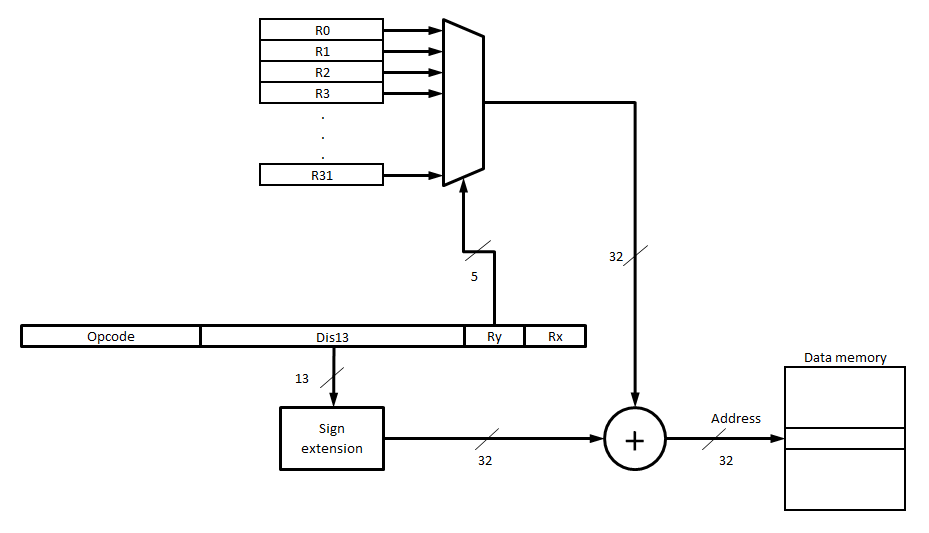
\includegraphics[scale=0.6]{./figures/eff_address.png}
\caption{Effective data memory address calculation.}
\end{figure}

\subsection{Instruction Memory}
\label{ssec:instruction_memory}

\begin{itemize}
   \item Instruction memory is read-only for the procesor. Read cycle takes only one clock period.
   \item Memory is organized in big-endian format.
   \item Only 32 bits single-word instructions are supported.
   \item An instruction can only be located in addresses multiple of 4.
   \item First 32 adresses (128 bytes) are reserved for exception vectors.
\end{itemize}
See figure \ref{fig:im_organization}

\begin{figure}
\begin{center}
\begin{bytefield}[bitwidth=0.9em]{40}
   \bitbox[]{8}{} & \bitbox[]{8}{+0} & \bitbox[]{8}{+1} & \bitbox[]{8}{+2} & \bitbox[]{8}{+3}\\
   \bitbox[]{8}{}
      & \bitbox[]{1}{\texttt{7}} & \bitbox[]{1}{\texttt{}} & \bitbox[]{1}{\texttt{}} & \bitbox[]{1}{\texttt{}}
      & \bitbox[]{1}{\texttt{}}  & \bitbox[]{1}{\texttt{}} & \bitbox[]{1}{\texttt{}} & \bitbox[]{1}{\texttt{0}}
      & \bitbox[]{1}{\texttt{7}} & \bitbox[]{1}{\texttt{}} & \bitbox[]{1}{\texttt{}} & \bitbox[]{1}{\texttt{}}
      & \bitbox[]{1}{\texttt{}}  & \bitbox[]{1}{\texttt{}} & \bitbox[]{1}{\texttt{}} & \bitbox[]{1}{\texttt{0}}
      & \bitbox[]{1}{\texttt{7}} & \bitbox[]{1}{\texttt{}} & \bitbox[]{1}{\texttt{}} & \bitbox[]{1}{\texttt{}}
      & \bitbox[]{1}{\texttt{}}  & \bitbox[]{1}{\texttt{}} & \bitbox[]{1}{\texttt{}} & \bitbox[]{1}{\texttt{0}}
      & \bitbox[]{1}{\texttt{7}} & \bitbox[]{1}{\texttt{}} & \bitbox[]{1}{\texttt{}} & \bitbox[]{1}{\texttt{}}
      & \bitbox[]{1}{\texttt{}}  & \bitbox[]{1}{\texttt{}} & \bitbox[]{1}{\texttt{}} & \bitbox[]{1}{\texttt{0}} \\
   \bitbox[]{8}{\texttt{0x00000000}} & \bitbox[ltb]{8}{Byte 3} & \bitbox[tb]{8}{Byte 2} & \bitbox[tb]{8}{Byte 1} & \bitbox[rtb]{8}{Byte 0}\\
   \bitbox[]{8}{\texttt{0x00000004}} & \bitbox[ltb]{8}{Byte 3} & \bitbox[tb]{8}{Byte 2} & \bitbox[tb]{8}{Byte 1} & \bitbox[rtb]{8}{Byte 0}\\
   \bitbox[]{8}{\texttt{0x00000008}} & \bitbox[ltb]{8}{Byte 3} & \bitbox[tb]{8}{Byte 2} & \bitbox[tb]{8}{Byte 1} & \bitbox[rtb]{8}{Byte 0}\\
   \bitbox[]{8}{\texttt{0x0000000C}} & \bitbox[ltb]{8}{Byte 3} & \bitbox[tb]{8}{Byte 2} & \bitbox[tb]{8}{Byte 1} & \bitbox[rtb]{8}{Byte 0}\\
   \bitbox[]{8}{}                    & \bitbox[lrt]{32}{} \\
   \bitbox[]{8}{}                    & \bitbox[lr]{32}{$\vdots$} \\
   \bitbox[]{8}{}                    & \bitbox[lrb]{32}{} \\
   \bitbox[]{8}{\texttt{0xFFFFFFFF}} & \bitbox[ltb]{8}{Byte 3} & \bitbox[tb]{8}{Byte 2} & \bitbox[tb]{8}{Byte 1} & \bitbox[rtb]{8}{Byte 0}\\
\end{bytefield}
\end{center}
\caption{Instruction memory organization.}
\label{fig:im_organization}
\end{figure}


\subsubsection{Program counter, branch and jump target addresses calculations}
\label{sssec:pc_branch_jump}
With instructions being 4 bytes long and unaligned access to instruction memory being not allowed, the effective instruction memory
address when stored in GPR's is given by bits 31 downto 2.
Branch or jump instructions that encode the address displacement in the corresponding field, also take advantage of this aligment
restriction, the two lower bits of the destination address are implicit (zeroes).

\subsection{Memory Timing Diagrams}
\label{ssec:memory_timing_diagrams}
\begin{figure}
\begin{center}
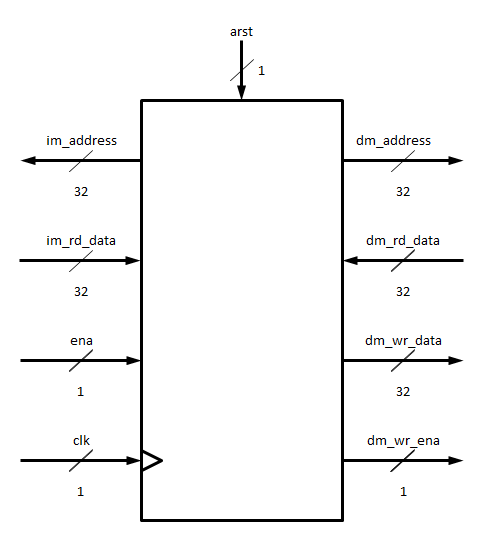
\includegraphics[scale=0.6]{./figures/interface.png}
\end{center}
\caption{Memory Port Interface.}
\label{fig:mem_port}
\end{figure}

\begin{figure}
\begin{center}
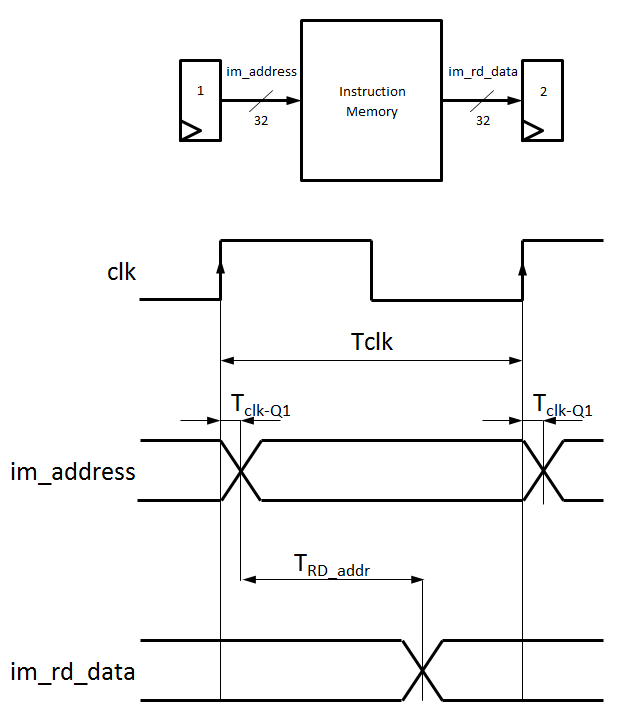
\includegraphics[scale=0.55]{./figures/im_rd_timing.png}
\end{center}
\caption{Instruction memory read cycle timing diagram.}
\label{fig:im_rd_timing}
\end{figure}

\begin{figure}
\begin{center}
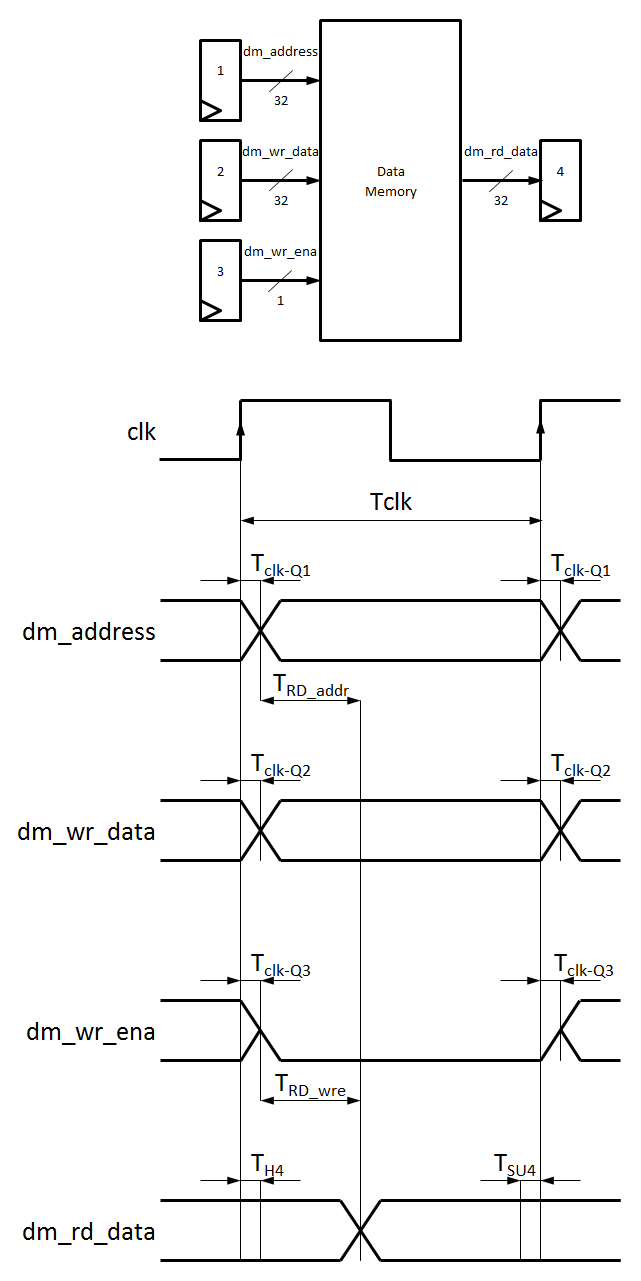
\includegraphics[scale=0.55]{./figures/dm_rd_timing.png}
\end{center}
\caption{Data memory read cycle timing diagram.}
\label{fig:dm_rd_timing}
\end{figure}

\begin{figure}
\begin{center}
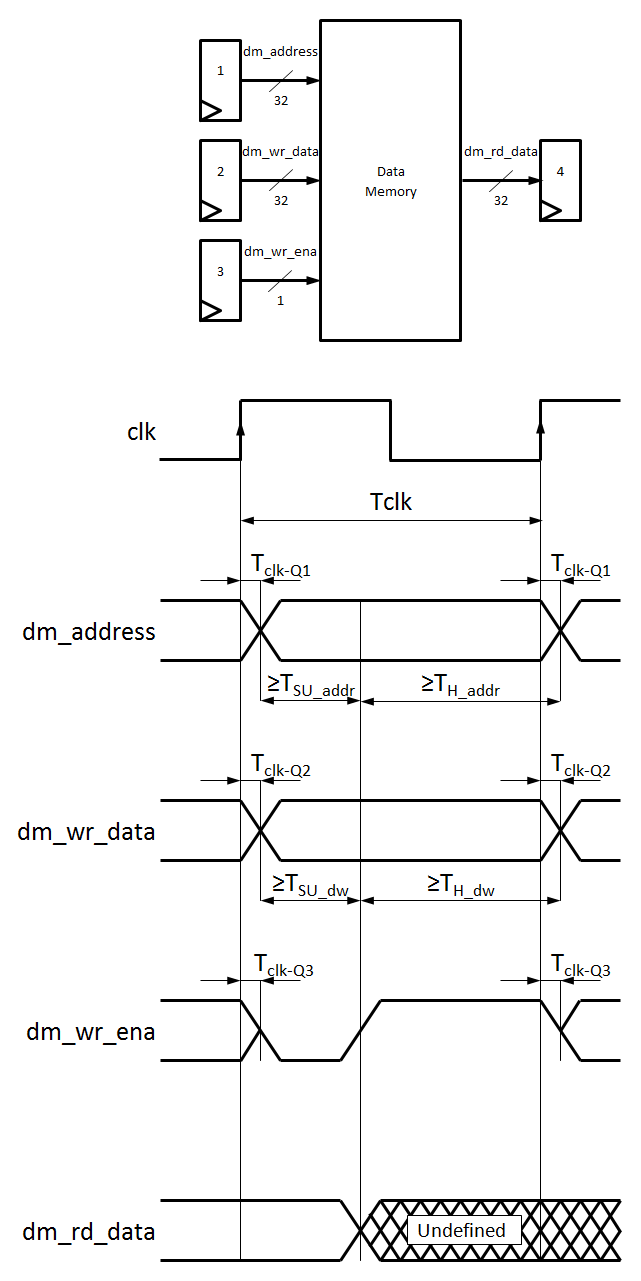
\includegraphics[scale=0.55]{./figures/dm_wr_timing.png}
\end{center}
\caption{Data memory write cycle timing diagram.}
\label{fig:dm_wr_timing}
\end{figure}

\begin{table}
\begin{center}
\begin{tabu} to \textwidth {|X[l]|X[l]|X[3,l]|}
\hline
\rowfont[c]\bfseries
\textbf{Parameter} & \textbf{Name} & \textbf{Description}\\
\hline
\hline
$T_{SU\_dw}$   & Write data setup time     & Minimum time to set dm\_wr\_data to a stable value before the rising edge of dr\_wr\_ena.\\
\hline
$T_{H\_dw}$    & Write data hold time      & Minimum time to hold dm\_wr\_data to a stable value after the rising edge of dr\_wr\_ena.\\
\hline
$T_{SU\_addr}$ & Address setup time        & Minimum time to set dm\_address to a stable value before the rising edge of dr\_wr\_ena.\\
\hline
$T_{H\_addr}$  & Address hold time         & Minimum time to hold dm\_address to a stable value after the rising edge of dr\_wr\_ena.\\
\hline
$T_{RD\_addr}$ & Read access time          & Maximum time taken by dm\_rd\_data to become valid after dm\_address changes.\\
\hline
$T_{RD\_wre}$  & Read access time          & Maximum time taken by dm\_rd\_data to become valid after dm\_wr\_ena goes low.\\
\hline
$T_{clk}$      & Clock period              & Period of time between two consecutive rising edges of clock signal.\\
\hline
$T_{clk-Q_i}$  & Clock to output time      & Propagation time of the register $i$.\\
\hline
$T_{SUi}$      & Register setup time       & Setup time of the register $i$.\\
\hline
$T_{Hi}$       & Register hold time        & Hold time of the register $i$.\\
\hline
\end{tabu}
\end{center}
\caption{Timing Parameters Description.}
\label{tbl:timing_paramerters}
\end{table}
